\documentclass{article}

\usepackage{amsthm}
\usepackage{amssymb,latexsym}
\usepackage{fancyhdr,amssymb}
\usepackage{mathtools}
\usepackage[shortlabels]{enumitem}
\usepackage{graphicx}
\usepackage{siunitx}


\title{Radon Transform}

\author{Gabriel Lapointe}


\begin{document}

\maketitle

\tableofcontents

\section{Introduction}
The scanner is generally represented by a cylinder in which there is a source where the positron is emitting a gamma pair. The detectors are located all around the scanner and are used to detect the gamma pairs emitted by the positron from the source.

However, while the positron is emitting a gamma pair, this positron may move enough to cause a banding error. This means that the lines traced by the gamma pair could be not colinear. This non-colinearity error induces a blur in the resolution of the image.

The objective is to model the reconstruction of the image without the blur causes by the non-colinearity error.  The first step will be to apply the Radon transform on the original image containing the blur in order to analyse the curve resulting from this transformation. The second step will be to reconstruct the image by applying the Radon-inverse transformation with the blur removed.


\section{Initial Geometry}
The objective is to define the initial geometry of a gamma pair in a scanner based on assumptions. 

\subsection{Assumptions}
The following assumptions are taken in order to simplify the model:
\begin{itemize}
	\item The scanner is represented as a circle (2 dimensions).
	\item The detectors size is infinitely small and are all around the circle.
	\item The source is located at the centre of the circle.
	\item The positron $e^+$ is kept at the source.
	\item The direction of the colinearity is uniform on $[0, \pi[$ because it is uniform in a sphere.
\end{itemize}


\subsection{Geometric Representation}
Let $\mathcal{C} \subset \mathbb{R}^2$ be the space represented by the circle of radius $r$. The space $\mathcal{C}$ is closed and bounded making it a compact space. 

In the figure \ref{fig:Scanner_Assumptions}, we represent the following details in function of our assumptions:

\begin{itemize}
	\item $S$ is the centre of the circle representing the source.
	\item $A$ and $B$ are 2 detectors chosen in the scanner.
	\item $(\gamma_1, \gamma_2)$ is the gamma pair emitted by the positron at the source $S$ and detected at $A$ and $B$.
	\item $\theta$ is the angle between the segments $\overline{S B}$ and $\overline{SP}$.
	\item $d\theta$ is the angle described by the bending error which is the angle between the segments $\overline{S B}$ and $\overline{S C}$. If $d\theta = 0$, the gamma pair is colinear.
	\item $\overline{D S}$ is perpendicular to the segment $\overline{A C}$.
\end{itemize}

\begin{figure}[ht!]
\centering
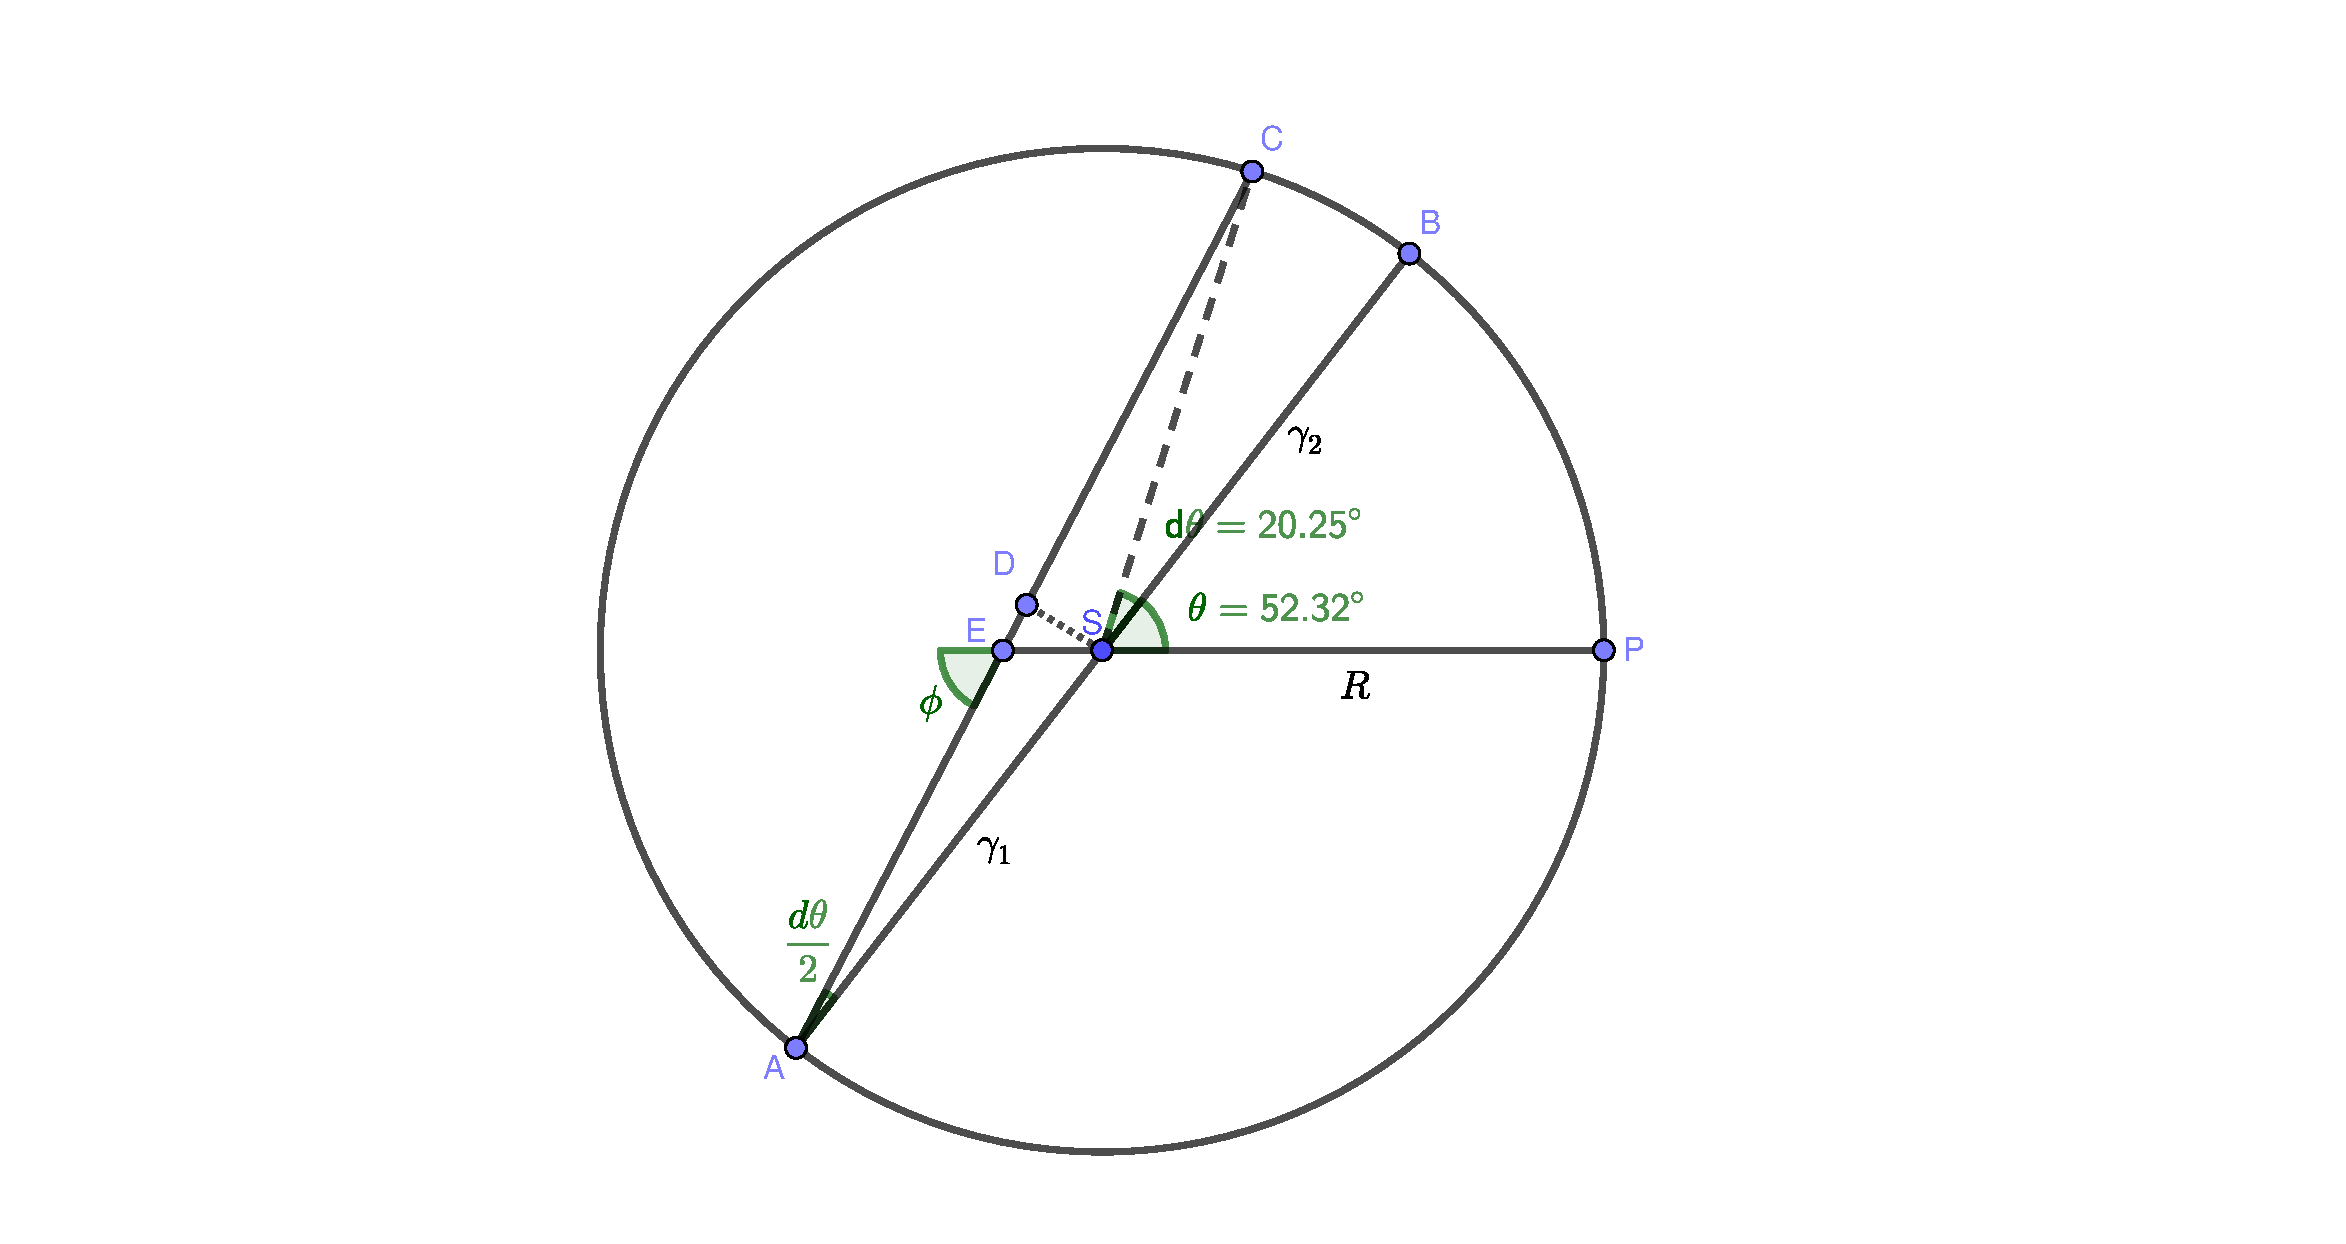
\includegraphics[width=121mm]{Images/Scanner_Blur.pdf}
\caption{2D-View of a scanner with 2 detectors with Blur
\label{fig:Scanner_Assumptions}}
\end{figure}

We represented the co-linearity error on the left side on the figure \ref{fig:Scanner_Assumptions} ($\theta + d\theta$), but it can be also on the right side ($\theta - d\theta$). We will consider $\theta + d\theta$ for our analysis.

According to the figure \ref{fig:Scanner_Assumptions}, we know that $\angle{BAC} = \frac{d\theta}{2}$ because of the inscribed angle property. Since $\angle{BSP} = \theta$, it holds that $\angle{ESA} = \theta$. We deduce that $\angle{AES} = \pi - \angle{ESA} - \angle{BAC}$. Therefore, we have that 
\begin{equation} \label{eq:Angle_Phi}
    \begin{aligned}
        \phi &= \angle{CES} \\
             &= \pi - (\pi - \angle{ESA} - \angle{BAC}) \\
             &= \angle{ESA} + \angle{BAC}) \\
             &= \theta + \frac{d\theta}{2}.
    \end{aligned}
\end{equation}

The segment $\overline{D S}$, perpendicular to the segment $\overline{A C}$, is the opposite side of the rectangle triangle $\Delta A D S$ where we know that the length of the segment $A S$ is $\left\| \mathbf{A} - \mathbf{S} \right\| = R$ the radius of the circle. Therefore, using the trigonometric property of the rectangle triangle, we have 
\begin{equation*}
    \sin \frac{d\theta}{2} = \frac{\left\| \mathbf{D} - \mathbf{S} \right\|}{R}
\end{equation*}
which is equivalent to
\begin{equation} \label{eq:Perp_Segment}
    \left\| \mathbf{D} - \mathbf{S} \right\| = R \sin \frac{d\theta}{2}.
\end{equation}


\section{Radon Transform}
The objective of using the Radon transform is to identify the blur described by the gamma pairs. The Radon transform determines the total density of a function $f$ described by an image.

\subsection{Cartesian to Polar Coordinates Without Blur}
Before going any further with the Radon transform, we have to define a mapping between the Cartesian coordinates $(x, y)$ to a polar coordinates.  

We know that the general equation of a line is given by 
\begin{equation} \label{eq:GeneralLine}
	ax + by - c = 0
\end{equation}
where $a,b,c \in \mathbb{R}$ are parameters of the line with $a^2 +  b^2 \neq 0$ and $(x, y) \in \mathbb{R}^2$ represents a point on the line. Since $a^2 +  b^2 \neq 0$, we can divide the equation \eqref{eq:GeneralLine} by $\sqrt{a^2 + b^2}$:
\begin{equation}
	\frac{a}{\sqrt{a^2 + b^2}} x + \frac{b}{\sqrt{a^2 + b^2}} y = \frac{c}{\sqrt{a^2 + b^2}}.
\end{equation}
On a geometric point of view, we see that $a$ is the opposite side or the rectangle triangle, $b$ the adjacent side and $c = \sqrt{a^2 + b^2}$ the hypotenuse. Therefore, we can draw a unit circle with any point $\left(\frac{a}{\sqrt{a^2 + b^2}}, \frac{b}{\sqrt{a^2 + b^2}}\right) = (\cos \theta, \sin \theta)$ where $\theta \in [0, 2\pi[$. If $u = \frac{c}{\sqrt{a^2 + b^2}}$, we obtain that
\begin{equation} \label{eq:u_coordinates}
	\langle (x, y), (\cos \theta, \sin \theta) \rangle = x \cos \theta + y \sin \theta = u.
\end{equation}
It follows that if $u$ and $\theta$ are fixed, it gives a line $l(u, \theta) \in \mathbb{R}^2$. Thus, $u$ and $\theta$ parameterize any line $l(u, \theta)$. Here, $u$ is the distance between the origin and the line $l$ and $\theta$ is the angle from the $x$-axis to the line $l$.

Also, we know that the perpendicular line to the line $l(u, \theta)$ is
\begin{equation}
\begin{aligned}
v &= x \cos \left(\theta + \frac{\pi}{2}\right) + y \sin \left(\theta + \frac{\pi}{2}\right) \\
  &= y \cos \theta - x \sin \theta
\end{aligned}
\end{equation}

To summarize, we rotated the Cartesian coordinates system by $\theta$ in order to obtain the polar coordinates system represented by the following $(u, v)$ axis (see figure \ref{fig:Polar_System}): 
\begin{equation} \label{eq:RotationSystem}
	\begin{bmatrix}
	    \cos \theta & \sin \theta \\
	    -\sin \theta & \cos \theta \\
	\end{bmatrix}
\cdot
	\begin{bmatrix}
  		x \\
  		y \\
	\end{bmatrix}
=
	\begin{bmatrix}
	    u \\
	    v \\
	\end{bmatrix}
\end{equation}

\begin{figure}[ht!]
\centering
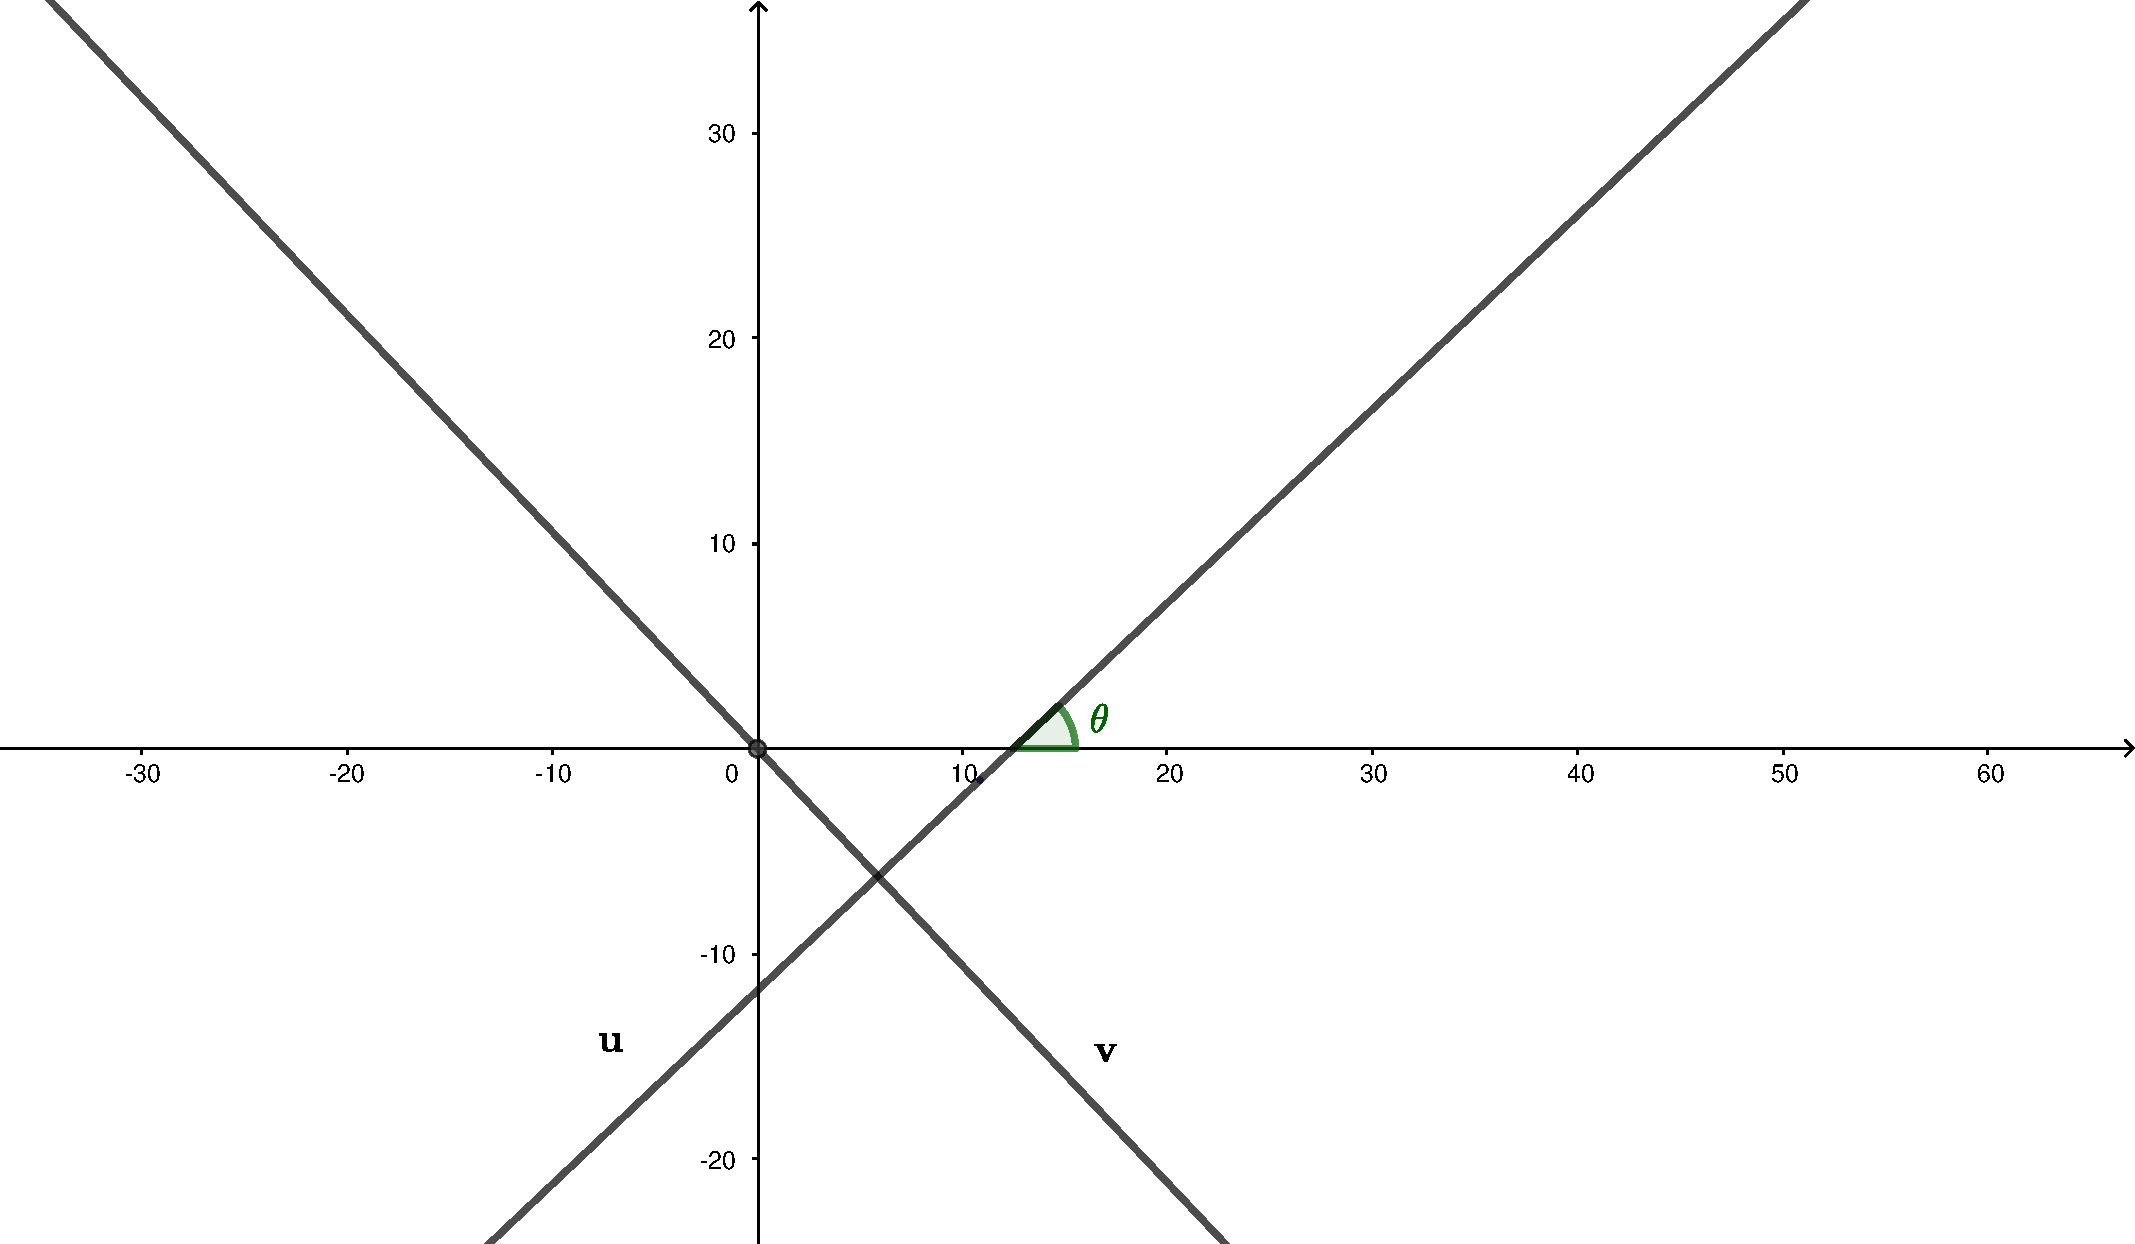
\includegraphics[width=120mm]{Images/PolarSystem.pdf}
\caption{Rotation of $\theta$ of the $(x, y)$ Cartesian coordinates
\label{fig:Polar_System}}
\end{figure}


\subsection{Cartesian to Polar Coordinates With Blur}
The objective is to change the Cartesian coordinates $(x, y)$ to polar coordinates considering the angle $d\theta$ induced by the blur this time.

Composing the rotation of $d\theta$ to the rotation of $\theta$ using the equation \eqref{eq:RotationSystem} gives:
\begin{equation} \label{eq:RotationSystemWithBlur}
\begin{aligned}
	\begin{bmatrix}
	  u^* \\
	  v^* \\
	\end{bmatrix}
	&=
	\begin{bmatrix}
	  \cos \theta & \sin \theta \\
	  -\sin \theta & \cos \theta \\
	\end{bmatrix}
\cdot
	\begin{bmatrix}
  		\cos \frac{d\theta}{2} & \sin \frac{d\theta}{2} \\
  		-\sin \frac{d\theta}{2} & \cos \frac{d\theta}{2} \\
	\end{bmatrix}
\cdot
	\begin{bmatrix}
  		x \\
  		y \\
	\end{bmatrix} \\
	&=
	\begin{bmatrix}
 		\cos \theta \cos \frac{d\theta}{2} - \sin \theta \sin \frac{d\theta}{2} & \cos \theta \sin \frac{d\theta}{2} + \sin \theta \cos \frac{d\theta}{2} \\
 		-(\sin \theta \cos \frac{d\theta}{2} + \cos \theta \sin \frac{d\theta}{2}) & \cos \theta \cos \frac{d\theta}{2} - \sin \theta \sin \frac{d\theta}{2} \\
	\end{bmatrix}
\cdot
	\begin{bmatrix}
  		x \\
  		y \\
	\end{bmatrix} \\
	&=
	\begin{bmatrix}
  		\cos(\theta + \frac{d\theta}{2}) & \sin(\theta + \frac{d\theta}{2}) \\
  		-\sin(\theta + \frac{d\theta}{2}) & \cos(\theta + \frac{d\theta}{2}) \\
	\end{bmatrix}
\cdot
	\begin{bmatrix}
  		x \\
  		y \\
	\end{bmatrix} \\
	&=
	\begin{bmatrix}
  		\cos \phi & \sin \phi \\
  		-\sin \phi & \cos \phi \\
	\end{bmatrix}
\cdot
	\begin{bmatrix}
  		x \\
  		y \\
	\end{bmatrix}
\end{aligned}
\end{equation}


\subsection{Radon Transform with Blur}
Now that we have rotated the $(x, y)$ coordinates to fit with our angle $\theta$ and knowing that we work in a closed and bounded space (meaning a compact space), we can use the Radon transform on the image described by $f(u, v)$ where $(u, v)$ represents all rotated (by $\theta$) pixels ($(x, y) \mapsto (u, v)$) in the image where $v$ is the line based on the angle $\theta + \frac{\pi}{2}$.

The Radon transform for an image $f$ with no blur is defined by
\begin{equation} \label{eq:RadonTransform_Clean}
\begin{aligned}
	\mathcal{R}(f(u, v)) &= \int_{-\infty}^{\infty} \int_{-\infty}^{\infty} f(u, v) \delta(u - x \cos \theta - y \sin \theta) du dv \\
						 &= \int_{-\infty}^{\infty} f(x \cos \theta + y \sin \theta, y \cos \theta - x \sin \theta) dx
\end{aligned}
\end{equation}
where $\delta$ is the Dirac delta function.

However, the Radon transformation described by the equation \eqref{eq:RadonTransform_Clean} assumes that the image described by $f$ is clean (no blur induced in the image or equivalently, the gamma pairs are all co-linear). In our case, we know that a blur is induced in the image. Therefore, if $f^*(u^*, v^*)$ is the image $f(u, v)$ with a blur induced, we are interested on finding $\mathcal{R}(f^*(u^*, v^*)) = g^*(u^*, v^*)$ where $g^*(u^*, v^*)$ is the sinogram resulting from the Radon transformation on $f^*(u^*, v^*)$. Recall that the angle described between the line $u^*$ and the $x$ axis is $\phi$ and the angle described between the line $v^*$ and the $x$ axis is $\phi + \frac{\pi}{2}$ because $v^* \bot u^*$.

Based on the system \eqref{eq:RotationSystemWithBlur} and equation \eqref{eq:Angle_Phi} on $\phi$, the Radon transform for an image $f^*$ induced by a blur is defined by
\begin{equation} \label{eq:RadonTransform_Blur}
\begin{aligned}
	\mathcal{R}(f^*(u^*, v^*)) &= \int_{-\infty}^{\infty} \int_{-\infty}^{\infty} f^*(u^*, v^*) \delta(u^* - x \cos \phi - y \sin \phi) du^* dv^* \\
						 &= \frac{1}{\pi} \int_{-\infty}^{\infty} f^*(x \cos \phi + y \sin \phi, y \cos \phi - x \sin \phi) dx \\
						 &= g^*(u^*, v^*).
\end{aligned}
\end{equation}

From our assumptions, we stated that $\theta \sim \mathcal{U}([0, \pi[)$. Thus, we have 
\begin{equation*}
    \mathbb{P}(\theta = \rho) = \frac{1}{\pi}
\end{equation*}
for all angles $\rho \in [0, \pi[$. This holds also for $\phi$ because $\phi$ is function of $\theta$. It explains why we divided by $\pi$.

%The probability to obtain an angle $\theta$ is calculated among the possible angles in a circle because it could be located everywhere in the circle based on $\theta$. We divided by $\pi$, not by $2\pi$ because it is possible to have an angle $\pi \leq \angle{A S P} < 2\pi$ or $0 \leq \angle{A S P} < \pi$. Hence, there is a duplicate which we do not want.

In virtue of \textbf{CITATION HERE}, the angle $d\theta$ induced by the blur follows a centered normal law: 
\begin{equation} \label{eq:dTheta_NormalLaw}
	d\theta \sim \mathcal{N}(0, \sigma^2)
\end{equation}
where 
\begin{align*}
    \sigma &= FWHM\left(\frac{\pi}{360}\right) \\
           &= \frac{\pi}{360 \times 2\sqrt{2 \ln 2}} \\
           &= 0.003705865.
\end{align*}

We saw with the equation \eqref{eq:Perp_Segment} that the segment $\overline{D S}$ (on the line $v^*$) is perpendicular to the segment $\overline{A C}$ represented by $u^*$. Thus, we can represent $v^*$ by the equation
\begin{equation} \label{eq:Perp_Sinus}
    v^*(d\theta) = R \sin{\frac{d\theta}{2}}
\end{equation}
where $\left\| \mathbf{D} - \mathbf{S} \right\| = R \sin{\left(\frac{\pi}{720}\right)}$ is the scaled version shown on the figure \ref{fig:Scanner_Assumptions}. 

From the equation \eqref{eq:Perp_Sinus}, we found the inverse of $v^*(d\theta)$:
\begin{equation*}
    d\theta = 2 \arcsin{\frac{v^*}{R}}.
\end{equation*}
Using $v^*$ as a random variable instead of $d\theta$, we obtain from \eqref{eq:dTheta_NormalLaw} that
\begin{equation*}
    \arcsin{\frac{v^*}{R}} \sim \mathcal{N}(0, (2\sigma)^2).
\end{equation*}
For simplification purposes and because $d\theta$ is very small (e.g. $d\theta \approx \frac{\pi}{360}$), we approximate $\sin{d\theta}$ by $d\theta$ because $\lim\limits_{d\theta \rightarrow 0} \sin{d\theta} = 0$. This implies that the equation \eqref{eq:Perp_Sinus} is simplified to the approximated linear equation 
\begin{equation} \label{eq:V_Approx}
    v^*(d\theta) \approx \frac{R}{2} d\theta.
\end{equation}
This is equivalent to $d\theta = \frac{2}{R}v^*$ because $R > 0$. It follows from \eqref{eq:dTheta_NormalLaw} that
\begin{equation*}
    v^* \sim \mathcal{N}\left(0, \left(\frac{R \sigma}{2}\right)^2\right).
\end{equation*}
Since $u^* \bot v^*$, we can say from the equation \eqref{eq:V_Approx} that $u^*(d\theta) \approx \frac{-2}{R} d\theta$ and that 
\begin{equation*}
    u^* \sim \mathcal{N}\left(0, \left(\frac{-2\sigma}{R}\right)^2\right).
\end{equation*}
In order to evaluate analytically the Radon transform of $f^*(u^*, v^*)$, we have to calculate the bi-variate Gaussian distribution for the random variable $(u^*, v^*) \in \mathbb{R}^2$. This distribution function is expressed as
\begin{equation} \label{eq:Multivariate_Gaussian}
    \mathbb{P}((u^*, v^*) = \mathbf{x}) = \frac{1}{2\pi \sqrt{\det \Sigma}} \exp\left\{\frac{-1}{2} (\mathbf{x} - \mu)^T \Sigma^{-1} (\mathbf{x} - \mu)\right\}
\end{equation}
where $\mathbf{x} = (u(x) = x\cos{\phi} + y\sin{\phi}, v(y) = -x\sin{\phi} + y\cos{\phi})$, $\mu = (0, 0)$ because it is centered and
\begin{equation} \label{eq:2D_Variance_Matrix}
    \Sigma = 
    \begin{bmatrix}
  		\sigma^2_{u^*} & Cov(u^*, v^*) \\
  		Cov(v^*, u^*) & \sigma^2_{v^*}
	\end{bmatrix}.
\end{equation}
Since $u^* \bot v^*$, we have that $Cov(u^*, v^*) = Cov(v^*, u^*) = 0$. Hence, the matrix \eqref{eq:2D_Variance_Matrix} is simplified to
\begin{equation*}
    \Sigma = 
    \begin{bmatrix}
  		\sigma^2_{u^*} & 0 \\
  		0 & \sigma^2_{v^*}
	\end{bmatrix}
\end{equation*}
which gives $\det \Sigma = \sigma^2_{u^*} \sigma^2_{v^*} > 0$ implying that $\Sigma$ is positive defined and
\begin{equation*}
    \Sigma^{-1} =
    \begin{bmatrix}
  		\frac{1}{\sigma^2_{u^*}} & 0 \\
  		0 & \frac{1}{\sigma^2_{v^*}}
	\end{bmatrix}.
\end{equation*}
We are now able to calculate
\begin{align*}
    \frac{-1}{2} (\mathbf{x} - \mu)^T \Sigma^{-1} (\mathbf{x} - \mu) &= \frac{-1}{2} (u, v) \begin{bmatrix}
  		\frac{1}{\sigma^2_{u^*}} & 0 \\
  		0 & \frac{1}{\sigma^2_{v^*}}
	\end{bmatrix}
	\begin{bmatrix}
  		u \\
  		v
	\end{bmatrix} \\
	&= \frac{-1}{2} \left(\frac{u^2}{\sigma^2_{u^*}} + \frac{v^2}{\sigma^2_{v^*}}\right).
\end{align*}
Therefore, the equation \eqref{eq:Multivariate_Gaussian} can be written for our case as
\begin{equation} \label{eq:Bivariate_Gaussian}
    \mathbb{P}((u^*, v^*) = \mathbf{x}) = \frac{1}{2\pi \sqrt{\sigma^2_{u^*} \sigma^2_{v^*}}} \exp\left\{\frac{-1}{2} \left(\frac{u^2}{\sigma^2_{u^*}} + \frac{v^2}{\sigma^2_{v^*}}\right)\right\}.
\end{equation}
This equation can be separated in a product of uni-variate distribution functions (noted $N$) on $u^*$ and $v^*$ where
\begin{equation*}
    \mathbb{P}(u^* = u) = \frac{1}{\sqrt{2\pi \sigma^2_{u^*}}} \exp\left\{ \frac{-u^2}{2\sigma^2_{u^*}}\right\}
\end{equation*}
and 
\begin{equation*}
    \mathbb{P}(v^* = v) = \frac{1}{\sqrt{2\pi \sigma^2_{v^*}}} \exp\left\{ \frac{-v^2}{2\sigma^2_{v^*}}\right\}.
\end{equation*}
Therefore, we obtain that 
\begin{equation} \label{eq:Product_Of_Gaussian}
    \mathbb{P}((u^*, v^*) = \mathbf{x}) = \mathbb{P}(u^* = u) \mathbb{P}(v^* = v).
\end{equation}

Substituting the equation \eqref{eq:Product_Of_Gaussian} in the Radon transform \eqref{eq:RadonTransform_Blur} gives
\begin{align}
    g^*(u^*, v^*) &= \frac{1}{\pi} \int_{-\infty}^{\infty} \mathbb{P}(u^* = u(x)) \mathbb{P}(v^* = v(y)) dx \\
                   &= \frac{1}{\pi} \mathbb{P}(v^* = v(y)) \int_{-\infty}^{\infty} \mathbb{P}(u^* = u(x)) dx \\
                   &= \frac{1}{\pi} \mathbb{P}(v^* = v(y)).
\end{align}

We conclude that if $d\theta \sim \mathcal{N}(0, \sigma^2)$, then the blur will follow also a centered normal law.

\end{document}